\documentclass{article}

\usepackage{booktabs}
\usepackage{tabularx}
\usepackage{hyperref}
\usepackage{graphicx}
\usepackage{float}

%% Comments

\usepackage{color}

\newif\ifcomments\commentstrue %displays comments
\newif\ifcomments\commentsfalse %so that comments do not display

\ifcomments
\newcommand{\authornote}[3]{\textcolor{#1}{[#3 ---#2]}}
\newcommand{\todo}[1]{\textcolor{red}{[TODO: #1]}}
\else
\newcommand{\authornote}[3]{}
\newcommand{\todo}[1]{}
\fi

\newcommand{\wss}[1]{\authornote{blue}{SS}{#1}} 
\newcommand{\plt}[1]{\authornote{magenta}{TPLT}{#1}} %For explanation of the template
\newcommand{\an}[1]{\authornote{cyan}{Author}{#1}}

%% Common Parts

\newcommand{\progname}{Sayyara} % PUT YOUR PROGRAM NAME HERE
\newcommand{\authname}{Team 31
\\ SFWRENG 4G06
\\ Christopher Andrade
\\ Alyssa Tunney
\\ Kai Zhu
\\ Ethan Vince-Budan
\\ Collin Kan
\\ Harsh Gupta} % AUTHOR NAMES                  

\usepackage{hyperref}
    \hypersetup{colorlinks=true, linkcolor=blue, citecolor=blue, filecolor=blue,
                urlcolor=blue, unicode=false}
    \urlstyle{same}

\title{User Guide\\\progname}

\author{\authname}

\date{\today}

\begin{document}

\begin{table}[hp]
\caption{Revision History} \label{TblRevisionHistory}
\begin{tabularx}{\textwidth}{llX}
\toprule
\textbf{Date} & \textbf{Developer(s)} & \textbf{Change}\\
\midrule
April 1, 2023 & Alyssa & Addition of Sayyara demo link, how to run source code\\
\end{tabularx}
\end{table}

\newpage

\maketitle

\newpage

\section{Using the Sayyara Application}

To use the various features on the Sayyara website, a video demo has been created to demonstrate the flow of a customer creating an account and signing in, and following the process to look up shops, and then create a quote request to send to the desired shops. There is also the view of the shop owner/employee when a customer sends them a quote request, and how the flow resumes from their point of view. The video demo can be found \href{https://www.youtube.com/watch?v=HzWQdQTp5Vs&feature=youtu.be}{here on YouTube}.

\section{Running the Sayyara Application}

The Sayyara application currently runs locally due to deployment not being part of the project's MVP. In order to run the source code, the user needs to have the \href{https://www.docker.com/}{Docker} application installed on their machine. Once Docker is installed, a terminal can be opened and navigated to the \texttt{src\textbackslash} directory of this repository where the \texttt{docker-restart.sh} script is located. After running this script, the Docker container should be populated as such:

\begin{figure}[H]
    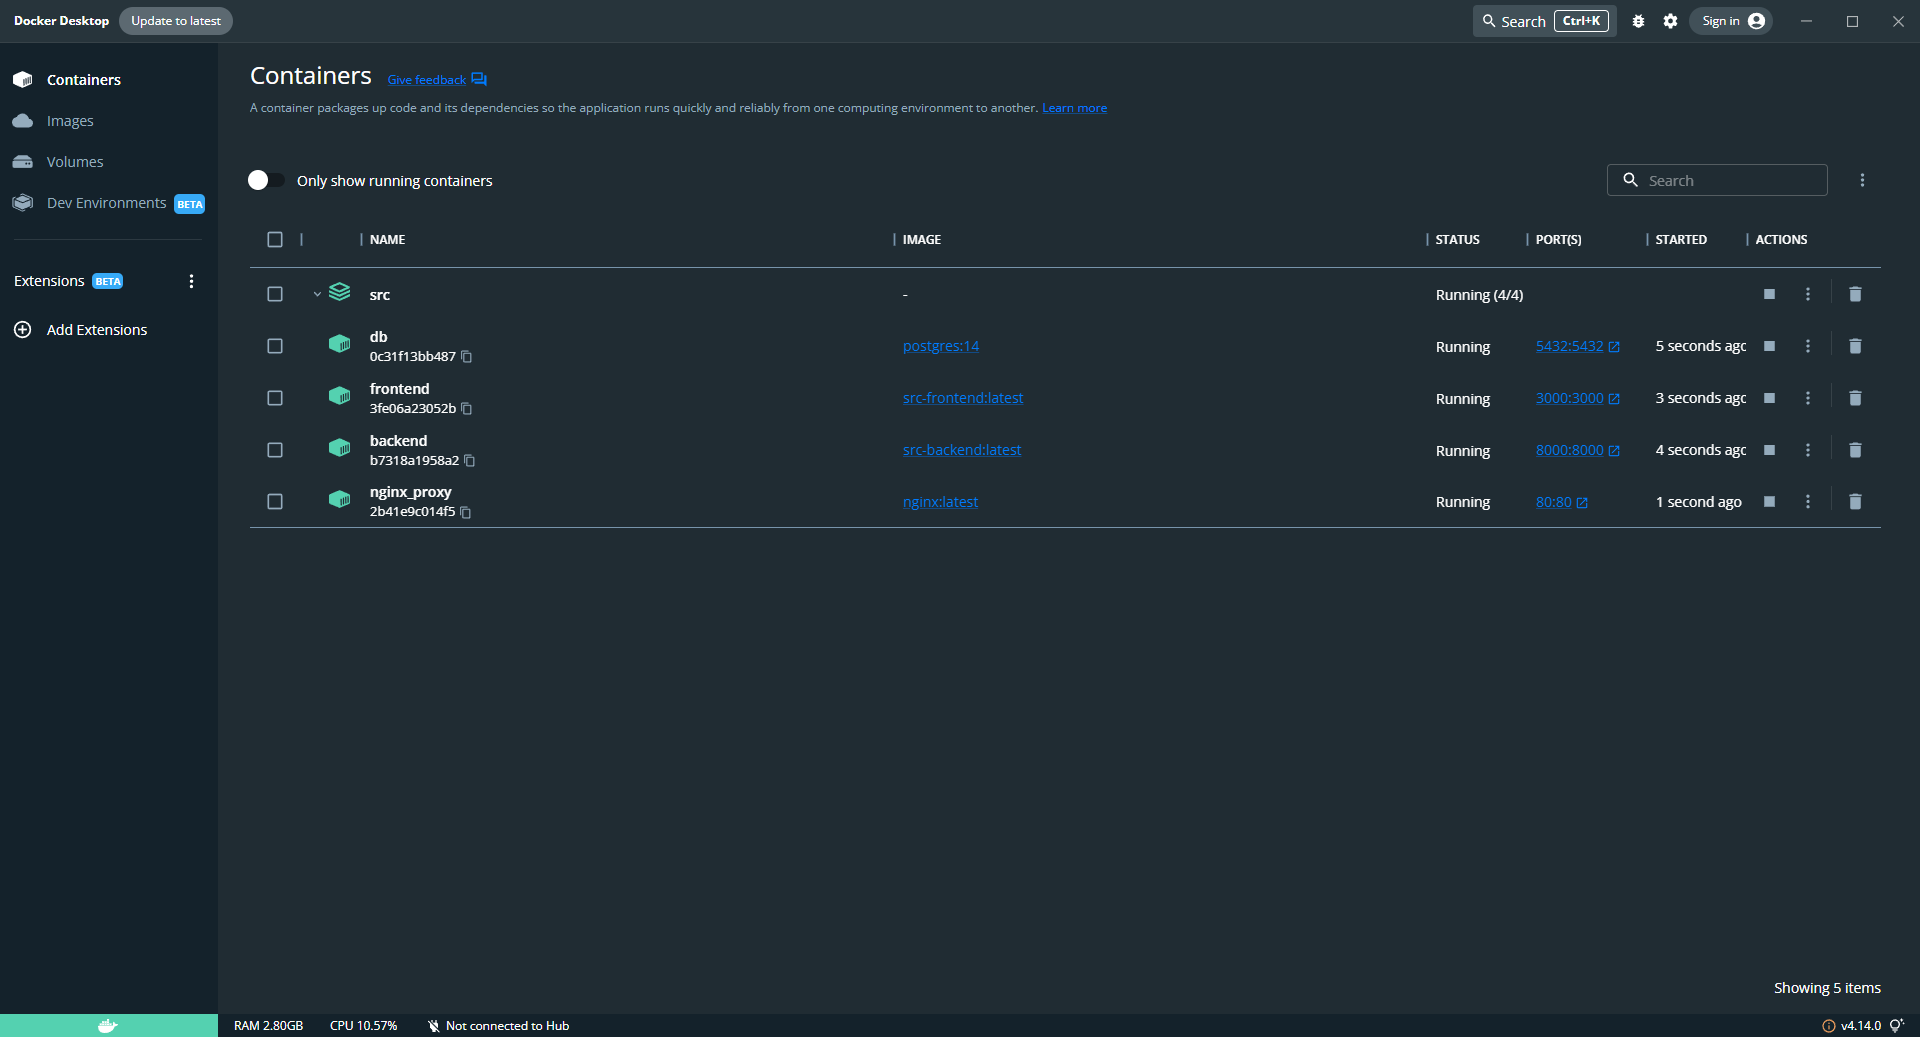
\includegraphics[width=1\textwidth]{images/docker.png}
    \caption{The Docker container housing the Sayyara application}
    \label{fig:my_label}
\end{figure}

\noindent Once running, the frontend can be found at \href{http://localhost/}{http://localhost/}. The backend APIs can be viewed at \href{http://localhost/api/swagger/}{http://localhost/api/swagger/}, and the related admin panel viewed at \href{http://localhost/api/admin/}{http://localhost/api/admin/} (Username: admin; Password: admin). Any additional information can be found in the README file located in \texttt{src\textbackslash}.

\subsection{Common Issues}

An issue that some of the team has run into when running the Docker container is that the \texttt{migrations.sh} script, located in \texttt{src\textbackslash backend\textbackslash} has compatibility issues due to being in CRLF mode. If VSCode is used, this can easily be modified to LF mode, which allows the backend in the Docker container to run properly.

\begin{figure}[H]
    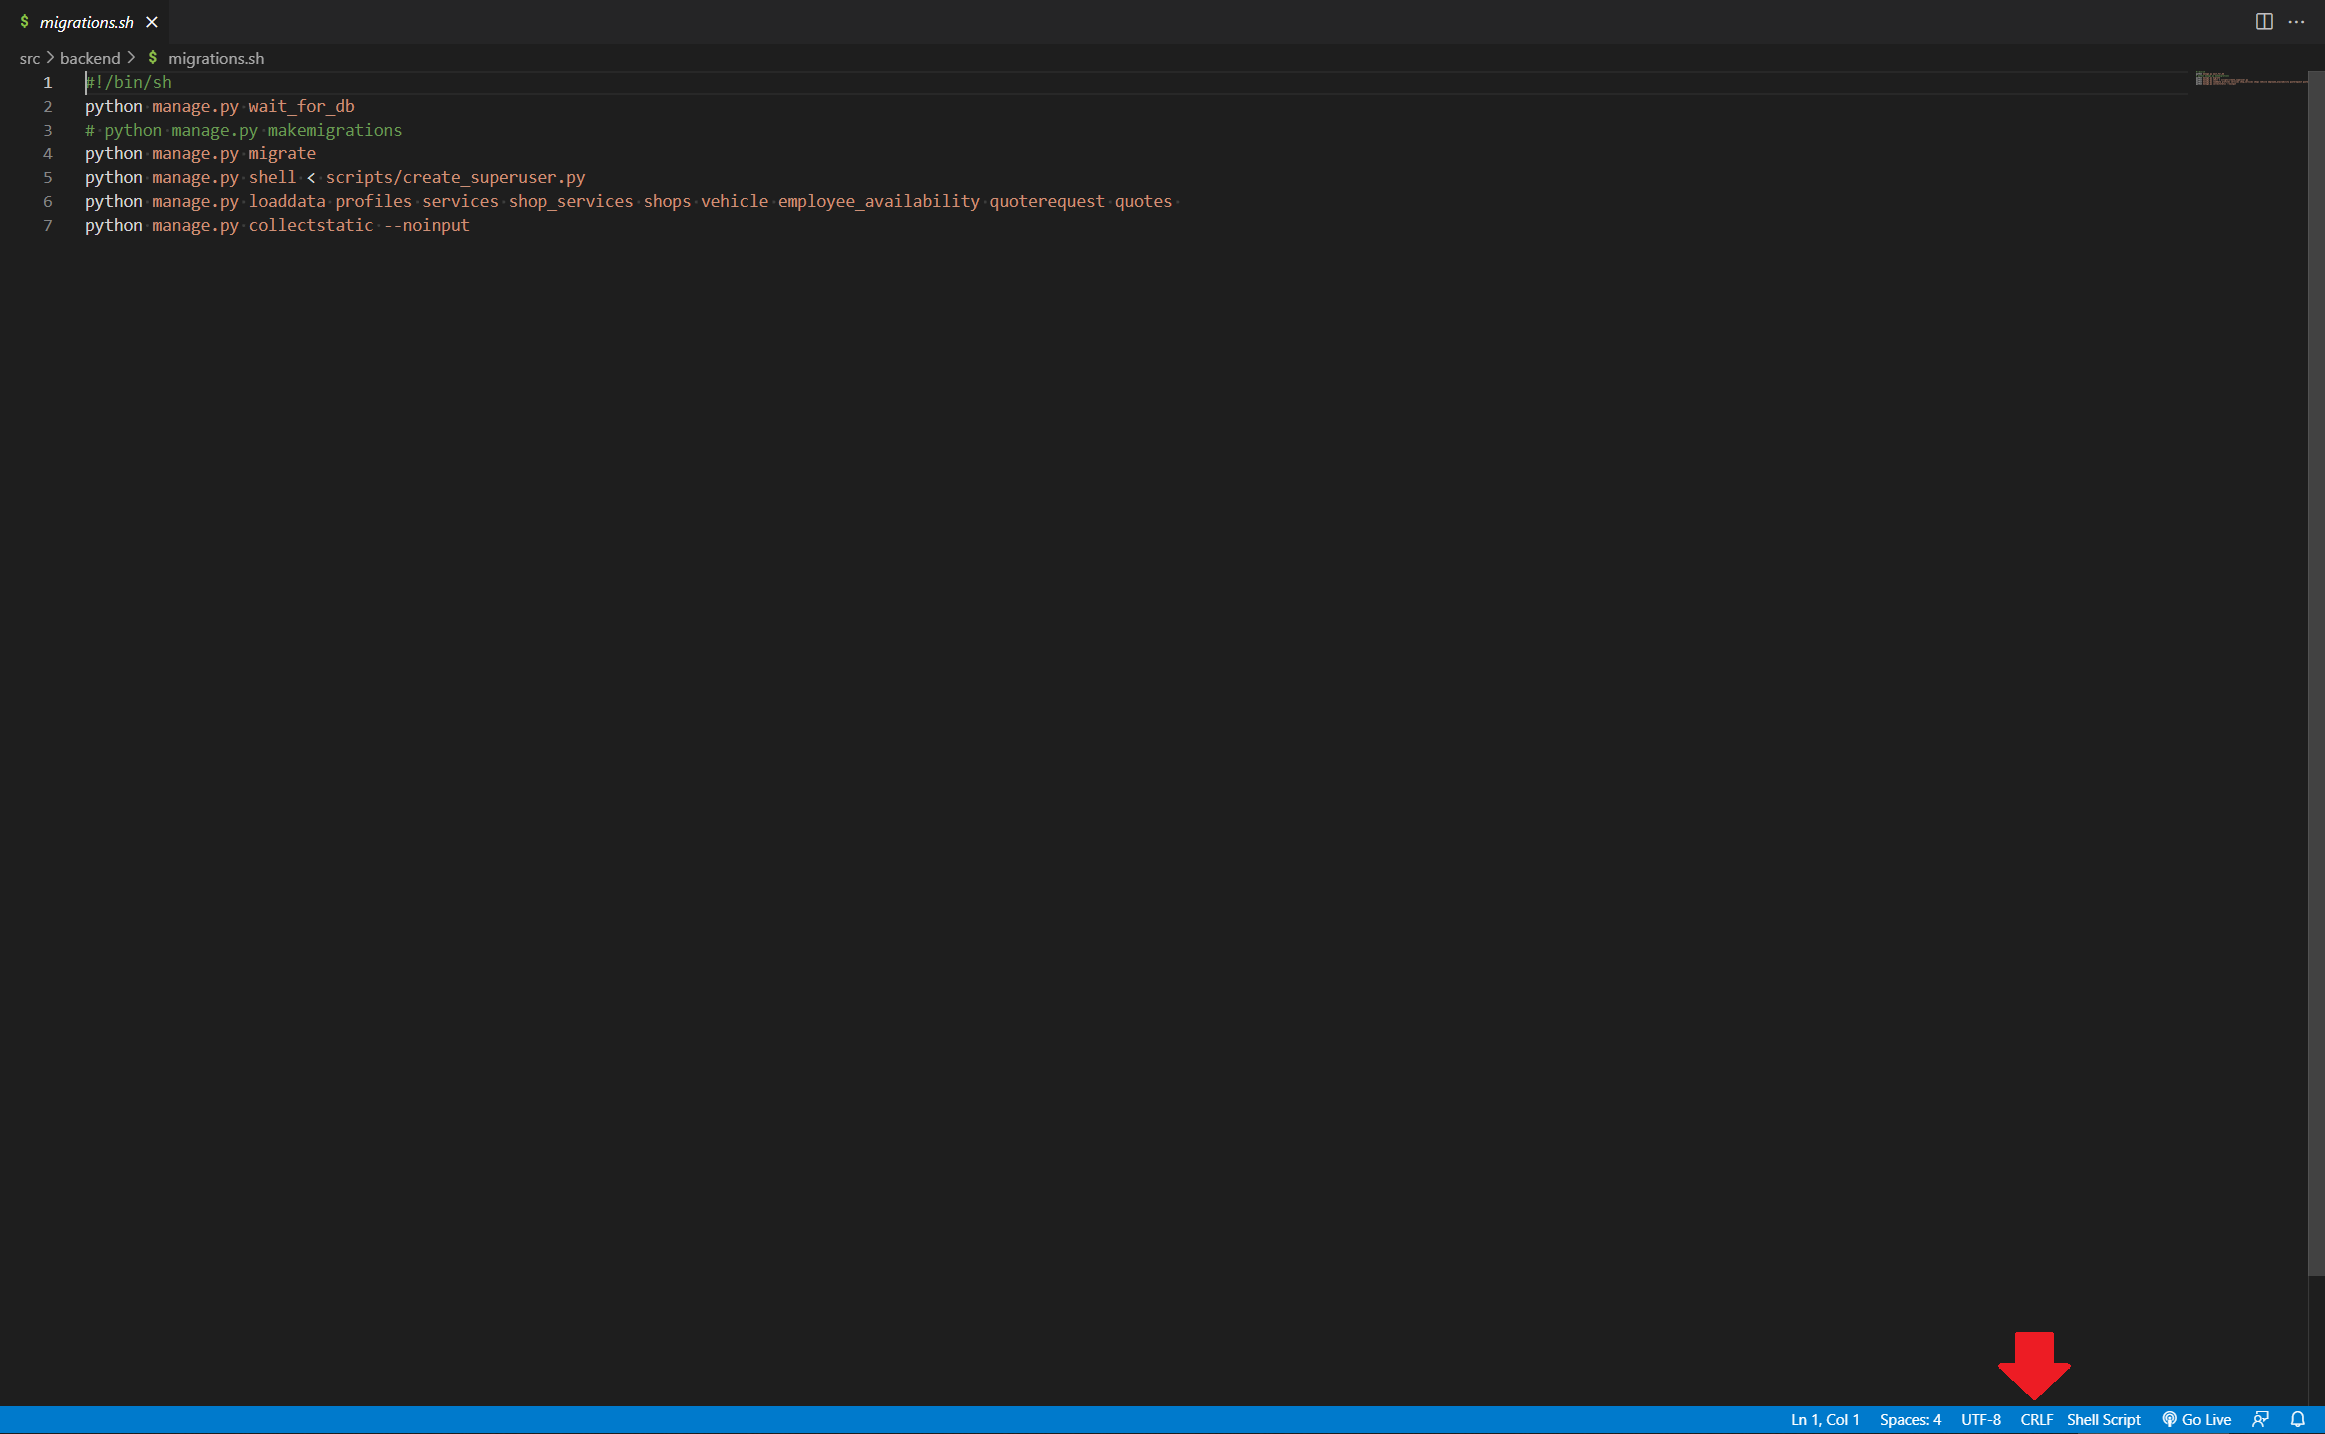
\includegraphics[width=1\textwidth]{images/crlf.png}
    \caption{migrations.sh running in CLRF}
\end{figure}

\begin{figure}[H]
    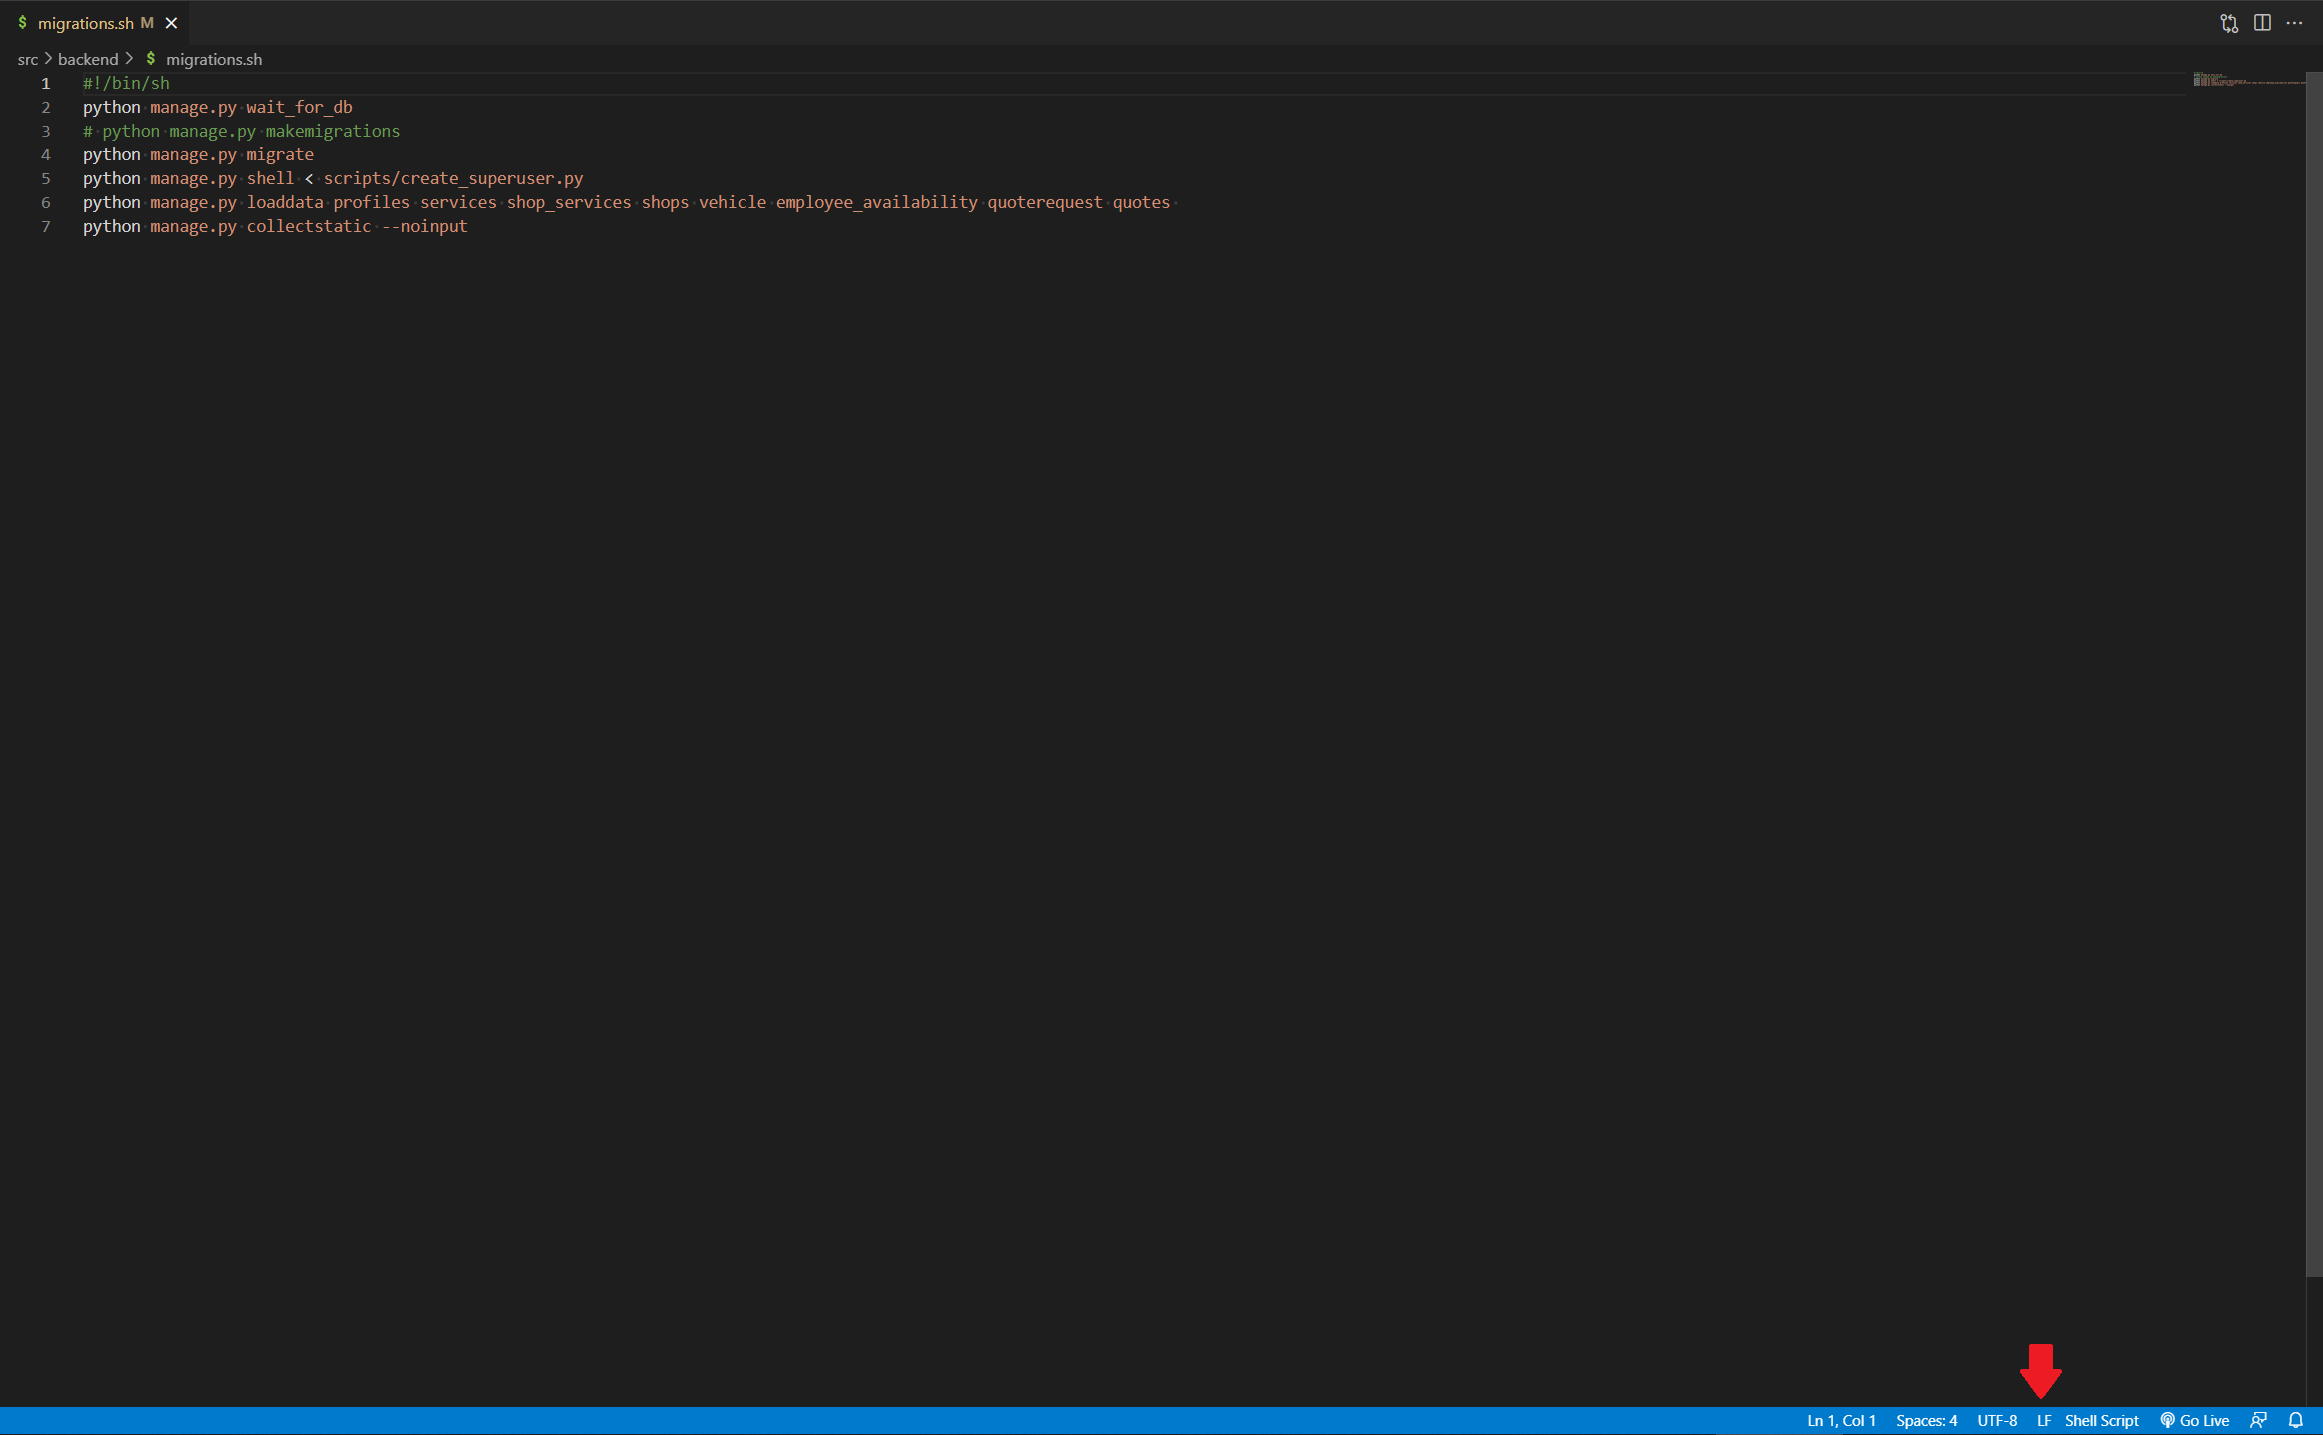
\includegraphics[width=1\textwidth]{images/lf.png}
    \caption{migrations.sh running in LF}
\end{figure}


\end{document}